\begin{frame}
\frametitle{I have done a terrible thing}

\begin{columns}
\column{0.35\textwidth}
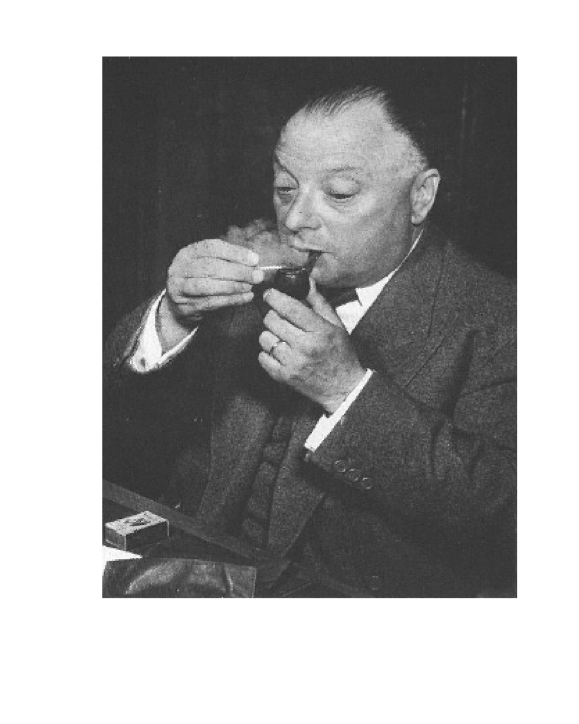
\includegraphics[scale=0.3]{pauli.png}
 
 \column{0.4\textwidth}
\begin{block}{}
Pauli neutral particles had to interact very weakly in order to escape undetected. Furthermore the mechanism by which the ``neutron" was produced was unspecified.

\vspace{0.5cm}

Pauli was unhappy with his brainchild. We wrote: ``I have  done a terrible thing. I have proposed a particle that cannot be detected. It is something no theorist should ever do". 

\end{block}
\end{columns}
\end{frame}
